\subsection{Measurements of $^{222}$Rn Concentration}
\label{secDelayedCoincidenceRn222}

The measurement of the radon concentration in the liquid xenon has been performed with two methods:  $\beta$-$\alpha$ delayed coincidence analysis of $^{214}$Bi-$^{214}$Po event pairs, and by spectral analysis of the $\alpha$-lines.

\begin{figure}[!h]
\centering
\subfigure[radon decay]{
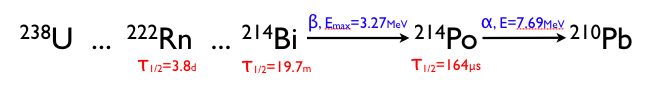
\includegraphics[width=0.6\linewidth]{plots/RnDC/DecayScheme_214.png}
\label{figRnDecayChain_1}}
\subfigure[thoron decay]{
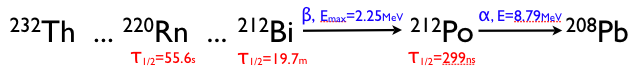
\includegraphics[width=0.6\linewidth]{plots/RnDC/DecayScheme_212.png}
\label{figRnDecayChain_2}}
\caption[Parts of the radon and thoron decay chains used for the delayed coincidence analysis]{Parts of the radon (a) and thoron (b) decay chains used for the delayed coincidence analysis.}
\label{figRnDecayChain}
\end{figure}

The decay scheme of $^{222}$Rn is shown in Fig.~\ref{figRnDecayChain_1}. The short lifetime of $^{214}$Po has been used to measure radon concentration in the liquid xenon target using {\it the delayed coincidence method}. A timing cut of $>$2~$\mu$s has been applied in order to avoid possible contribution from $^{212}$Bi-$^{212}$Po event pairs from thoron ($^{220}$Rn) decays with a shorter delay time (Fig.~\ref{figRnDecayChain_2}). 

\begin{floatingfigure}[lh]{0.475\textwidth}
%\begin{figure}[!h]
\centering
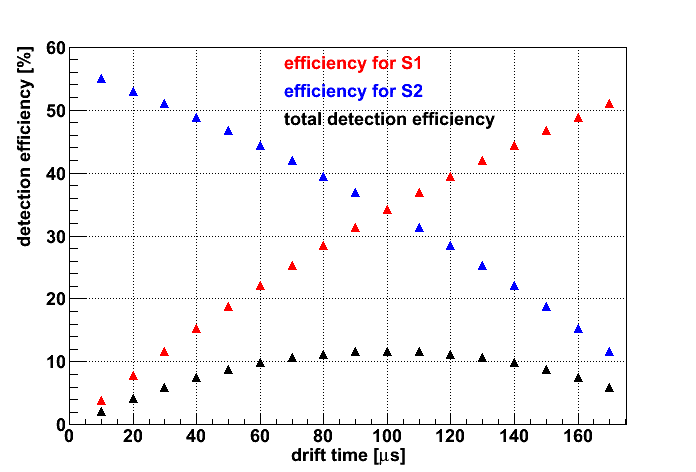
\includegraphics[width=0.475\linewidth]{plots/RnDC/detEff_total.png}
\caption[Detection efficiency for $\alpha$-interactions from $^{214}$Po decay]{Detection efficiency for $\alpha$-interactions from $^{214}$Po decay.}
\label{figBiPoDetEff}
%\end{figure}
\end{floatingfigure}

The DAQ is triggered by an S1 pulse from the electron produced in the $\beta$-decay of $^{214}$Bi with an endpoint of 3.27~MeV, since it is certainly above the S2 trigger threshold of $\sim$300~PE. 
The decay of $^{214}$Bi is followed by an $\alpha$-decay of $^{214}$Po with an energy of 7.7~MeV and a half-life of 164~$\mu$s. 
The efficiency to detect S1 and S2 pulses from the $\beta$ and $\alpha$ interactions are limited by the time gate:

\begin{equation}
\label{eqDetectionEfficiency}
eff = \frac{\int_{t_{1}}^{t_{2}}e^{-\lambda t}dt  }{ \int_{0}^{inf}e^{-\lambda t}dt },
\end{equation}
where $\lambda$ - decay constant of the $^{214}$Po isotope.
Since the peak finder algorithm does not search for an S1 after an S2 peak (see Section~\ref{secDAQ}), the time gate for an S1 from the $\alpha$-interaction from $^{214}$Po decay is limited by the drift time between the S1 and S2 from the $\beta$-interaction ($t_{2}$). The lower bound for the time gate ($t_{1}$) is limited by 2~$\mu$s. The time window to detect the S2 from an $\alpha$-interaction is between the drift time ($t_{1}$) and the length of the data acquisition window ($t_{2}$). 
The calculated detection efficiencies are shown in Fig.~\ref{figBiPoDetEff}. The cumulative efficiency to detect both S1 and S2 from $^{214}$Po is below 10\%. Therefore, the delayed coincidence analysis has been performed on the S1 signal only, with the average acceptance of 35\%.

Examples of the waveforms of $^{214}$Bi-$^{214}$Po candidate events are shown in Fig.~\ref{figBiPoWF}. The measured delay time, shown in Fig.~\ref{figBiPoSpectra_1}, is (233$\pm$10)~$\mu$s, in very good agreement with the expectation of 236~$\mu$s.

\begin{figure}[!b]
\centering
\subfigure[]{
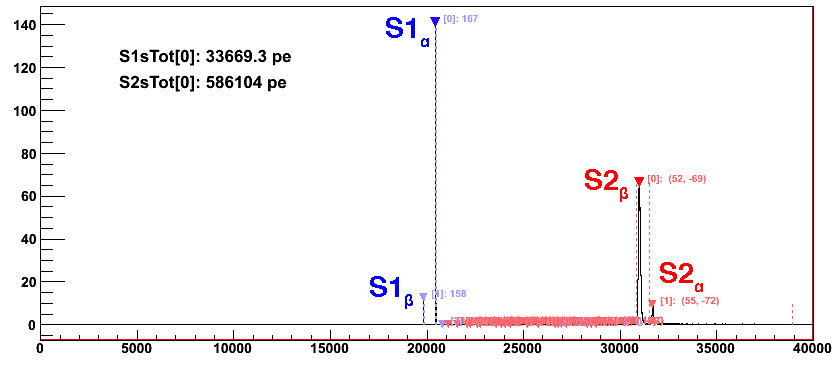
\includegraphics[width=0.475\linewidth]{plots/RnDC/event1_withLabels.png}
\label{figBiPoWF_1}}
\subfigure[]{
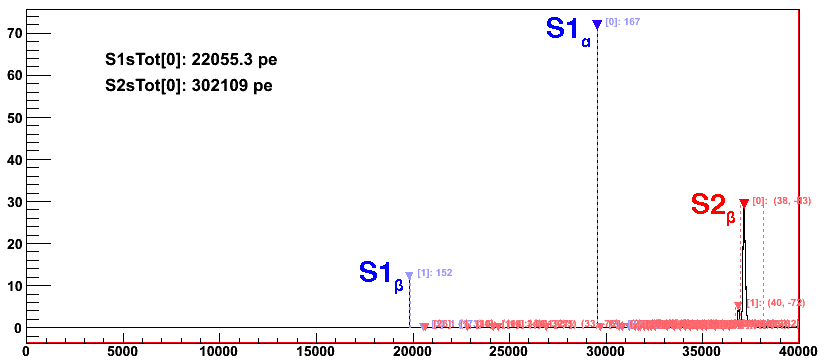
\includegraphics[width=0.475\linewidth]{plots/RnDC/event3_withLabels.png}
\label{figBiPoWF_2}}
\caption[Waveforms of $^{214}$Bi-$^{214}$Po candidate events tagged with the delayed coincidence analysis]{Waveforms of $^{214}$Bi-$^{214}$Po candidate events tagged with the delayed coincidence analysis: (a) - both S1 and S2 from $\alpha$ have been detected; (b) - S2 from $\alpha$-interaction is not present in the waveform due to large drift time.}
\label{figBiPoWF}
\end{figure}

Decays of $^{222}$Rn in the liquid xenon have been simulated with GEANT4, assuming a uniform distribution in the entire target volume. The Monte Carlo expectation has been compared to the energy spectrum of the tagged $\beta$ and $\alpha$ interactions reconstructed from the S1 signal. The simulation has been normalized to the height of the maximum bin in the measured spectrum. The agreement of the simulated and measurement spectra is remarkable and shown in Fig.~\ref{figBiPoSpectra_2}.

\begin{figure}[!b]
\centering
\subfigure[]{
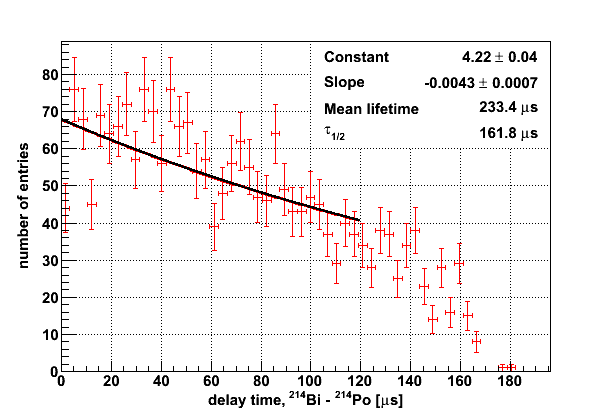
\includegraphics[height=0.33\linewidth]{plots/RnDC/TimeDif_Bi214-Po214.png}
\label{figBiPoSpectra_1}}
\subfigure[]{
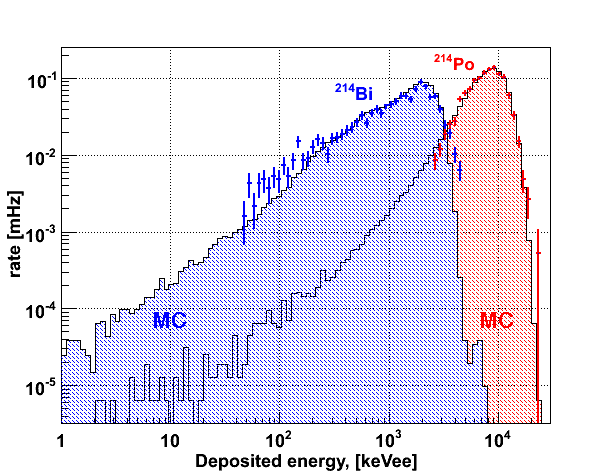
\includegraphics[height=0.33\linewidth]{plots/RnDC/Bi214-Po214_MCandDATA_withLabels.png}
\label{figBiPoSpectra_2}}
\caption[Delay time between the tagged $^{214}$Bi and $^{214}$Po decays, and comparison of their simulated and measured energy spectra]{Delay time between the tagged $^{214}$Bi and $^{214}$Po decays (a), and comparison of their simulated and measured energy spectra (b). The shaded histograms represent the Monte Carlo spectra. The energy cut to select $\beta$-events in the measured data is from 40~keV to 4~MeV, and the range for $\alpha$ is 2.5$-$20~MeV.}
\label{figBiPoSpectra}
\end{figure}

\begin{figure}[!b]
\centering
\subfigure[run07]{
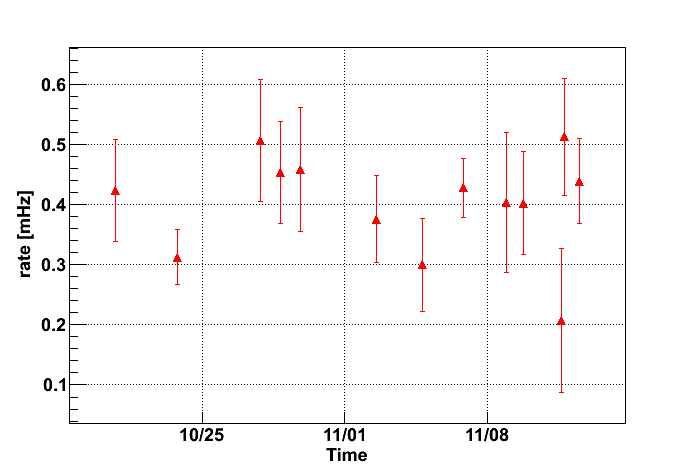
\includegraphics[width=0.475\linewidth]{plots/RnDC/rate_vs_time_run07_DelayedCoincidence.png}
\label{figRateDC_1}}
\subfigure[run08]{
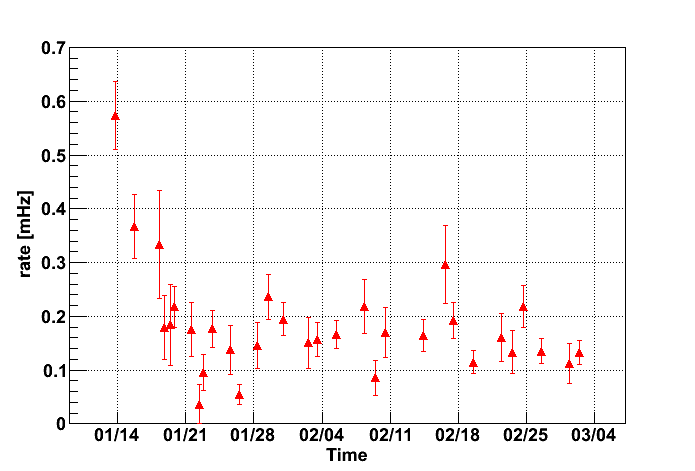
\includegraphics[width=0.475\linewidth]{plots/RnDC/rate_vs_time_run08_DelayedCoincidence.png}
\label{figRateDC_2}}
\caption[Rate of the $^{214}$Bi-$^{214}$Po decays measured with delayed coincidence analysis in run07 and run08]{Rate of the $^{214}$Bi-$^{214}$Po decays measured with delayed coincidence analysis in run07 (a) and run08 (b).}
\label{figRateDC}
\end{figure}

The time evolution of the rate of $^{214}$Bi-$^{214}$Po decays measured with the delayed coincidence analysis is shown in Fig.~\ref{figRateDC_1} and Fig.~\ref{figRateDC_2}, for the commissioning run in Fall 2009 (run07) and for the first science run (run08), respectively. 
The average rate in run07 is 0.4~mHz. Taking into account the average S1 detection efficiency of 35\% shown in Fig.~\ref{figBiPoDetEff}, and the acceptance of the energy cuts of $\sim$30\%, estimated from the comparison of the measured and simulated energy spectra shown in Fig.~\ref{figBiPoSpectra_2}, the cumulative detection efficiency for the delayed coincidence analysis is $\sim$10\%.
The corresponding $^{222}$Rn concentration is $\sim$20~$\mu$Bq/kg. This value is similar to that reported for the XMASS prototype detector~\cite{XmassRadon}. 
An increase of radon concentration at the beginning of the time period shown in Fig.~\ref{figRateDC_2} was due to an air leak during maintenance work on the gas recirculation, prior to the start of the data acquisition period. This additional radon decays with a characteristic half-life time of 2.8~days down to a level about two times lower than in run07, due to purification with the distillation column.

\begin{figure}[!t]
\centering
\subfigure[]{
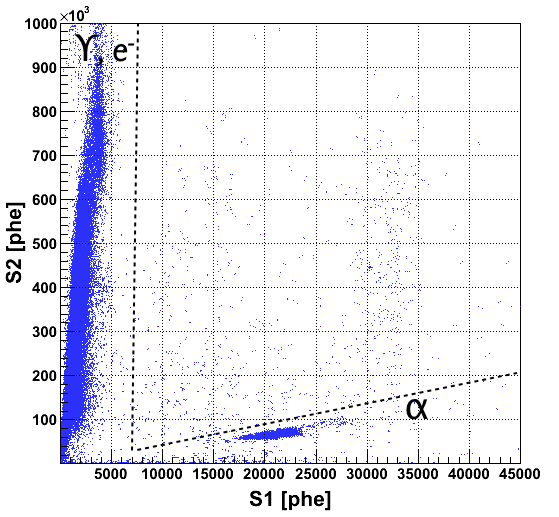
\includegraphics[height=0.35\linewidth]{plots/RnDC/S2_vs_S1_run08_FV30.png}
\label{figS2S1alpha_1}}
\subfigure[]{
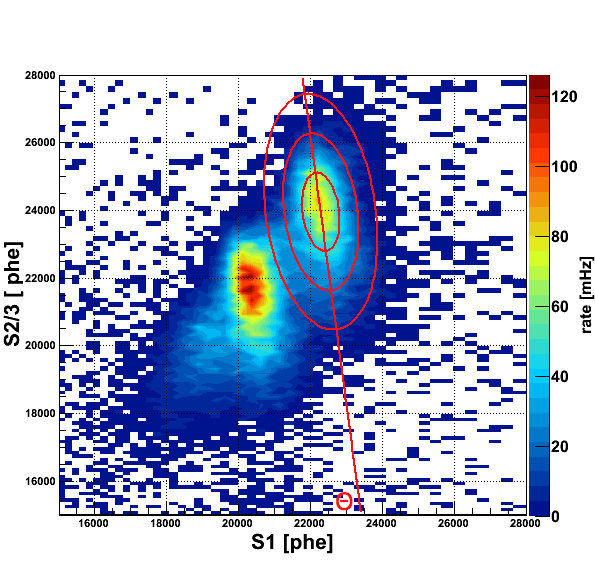
\includegraphics[height=0.38\linewidth]{plots/RnDC/S2const3_vs_S1_FitAlpha2nd_mod.png}
\label{figS2S1alpha_2}}
\caption[Prompt (S1) and proportional (S2) scintillation signals for different types of particles, and an elliptical Gaussian fit to the $^{218}$Po peak]{Prompt (S1) and proportional (S2) scintillation signals for different types of particles (a), and a zoom into the region of $\alpha$-interactions with an elliptical Gaussian fit to the $^{218}$Po peak (b).}
\label{figS2S1alpha}
\end{figure}

\begin{figure}[!b]
\centering
\subfigure[run07]{
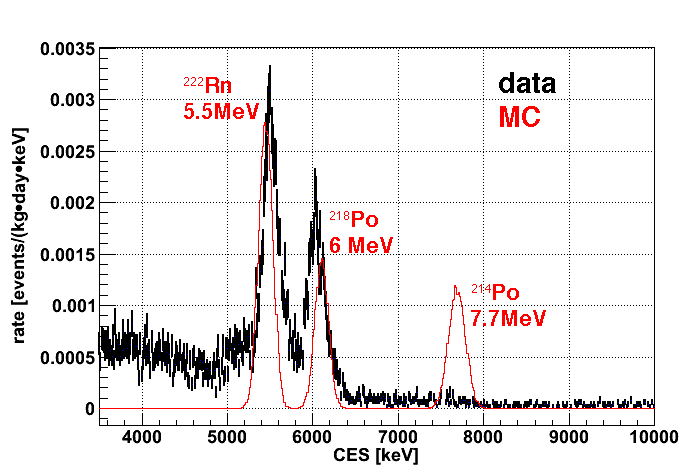
\includegraphics[width=0.475\linewidth]{plots/RnDC/MCdata_Rn222_2ndPeak_withLabels2.png}
\label{figCESalpha_1}}
\subfigure[run08]{
%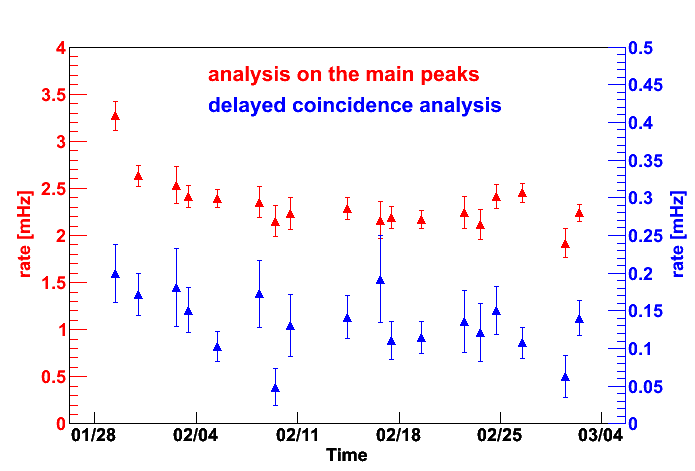
\includegraphics[width=0.475\linewidth]{plots/RnDC/2pads_RateComparison_run08_lowRn.png}
\includegraphics[width=0.475\linewidth]{plots/RnDC/BothMethods_run08.png}
\label{figCESalpha_2}}
\caption[Measured and simulated energy spectra for $\alpha$-events from $^{222}$Rn decays in the liquid xenon target volume, and comparison of the radon concentration measured with both methods]{(a) - measured and simulated energy spectra for $\alpha$-events from $^{222}$Rn decays in the liquid xenon target volume. The measured spectrum is shown in combined energy scale. The Monte Carlo spectrum is convoluted with the energy resolution of 1.7\%. The measured $^{222}$Rn and $^{218}$Po peaks are in a good agreement with the simulation. The absence of $^{214}$Po peak in the measured energy spectrum is due to low total detection efficiency of $<$10\%, compared to almost 100\% for the other $\alpha$-peaks. The radon concentration inferred from the fit is 21~$\mu$Bq/kg. (b) - rate of the $^{222}$Rn decays measured with spectral analysis of $\alpha$-lines and $\beta$-$\alpha$ delayed coincidence method in the first science run (run08).}
\label{figCESalpha}
\end{figure}

The prompt and proportional scintillation signals for the different types of particles are shown in a scatter plot in Fig.~\ref{figS2S1alpha_1}. The ionization yield for alphas is much lower than for $\gamma$-rays or relativistic electrons, which  provides a possibility to identify $\alpha$-interactions, and to perform a {\it spectral analysis}.
Fig.~\ref{figS2S1alpha_2} shows a zoom into the $\alpha$ region. The distribution has been fitted with an elliptical Gaussian function, and the anti-correlation angle has been extracted from the fit. The fit  parameters have been used to define the combined energy scale as described in Section~\ref{secCES}:
\begin{equation}
\mathrm{CES}_{\alpha}\ \text{[keV]} = \mathrm{S}1_{\mathrm{total}} \cdot 3.159 + \mathrm{S}2_{\mathrm{bottom}} \cdot 0.473.
\end{equation}

The resulting energy spectrum is compared to the one obtained from a Monte Carlo simulation of $^{222}$Rn decays in the liquid xenon in Fig.~\ref{figCESalpha_1}. The simulation has been scaled to 21~$\mu$Bq/kg of $^{222}$Rn distributed uniformly within the liquid xenon target. The peaks correspond to $\alpha$-interactions from $^{222}$Rn (5.5~MeV), $^{218}$Po (6~MeV), and $^{214}$Po (7.7~MeV) decays. The $^{214}$Po peak is not present in the measured spectrum due to the very low efficiency to detect both S1 and S2 from this interaction ($<$10\%, see Fig.~\ref{figBiPoDetEff}), compared to almost 100\% for the other $\alpha$-peaks. 
%The $^{222}$Rn peak might have a possible contribution from 5.3~MeV from $^{210}$Po decay, if concentration of $^{210}$Pb is significant. 
The tail on the left is from high energy $\gamma$-rays. Their energy is not correctly reconstructed due to large difference between ionization and scintillation yield for $\gamma$ and $\alpha$.

The results of both analysis methods applied to the first science run (run08) are shown in Fig.~\ref{figCESalpha_2}. Taking into account large error bars of the delayed coincidence measurement, the trend is the same. However, the spectroscopy analysis of the $^{222}$Rn and $^{218}$Po $\alpha$-lines provides an order of magnitude higher sensitivity, due to low detection efficiency for $^{214}$Po events in the $\beta$-$\alpha$ delayed coincidence analysis. 


%\begin{figure}[!h]
%\centering
%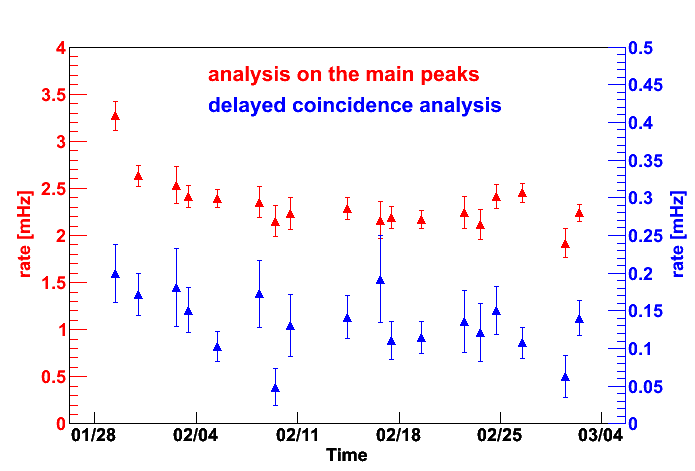
\includegraphics[width=0.475\linewidth]{plots/RnDC/2pads_RateComparison_run08_lowRn.png}
%\caption{Rate of the $^{222}$Rn decays measured with spectral and delayed coincidence analyses.}
%\label{figRateBothMethods}
%\end{figure}

%\begin{figure}[!h]
%\centering
%\subfigure[]{
%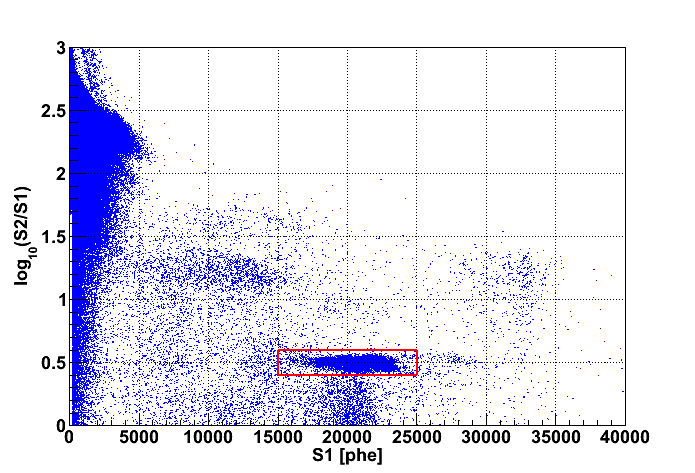
\includegraphics[width=0.475\linewidth]{plots/RnDC/logS2S1_vs_S1_linear_alpha1cut.png}
%\label{figAlphaBoxCut_1}}
%\subfigure[]{
%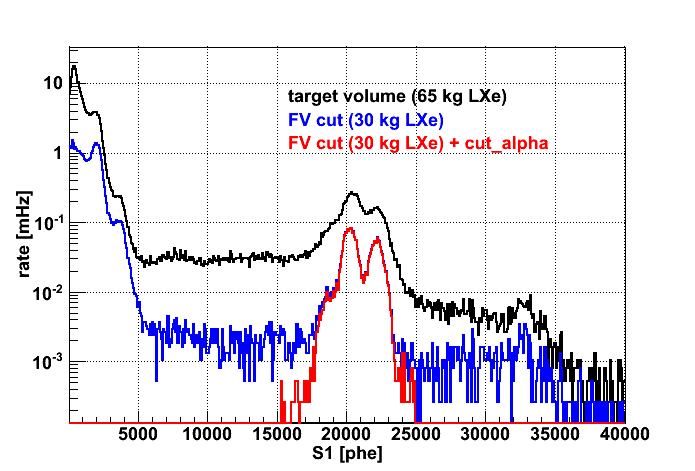
\includegraphics[width=0.475\linewidth]{plots/RnDC/S1phe_with_alpha1_FV30.png}
%\label{figAlphaBoxCut_2}}
%\caption{Selection of the alpha events with a cut on S1 and S2 anti-correlation.}
%\label{figAlphaBoxCut}
%\end{figure}


%\begin{figure}[!h]
%\centering
%\subfigure[]{
%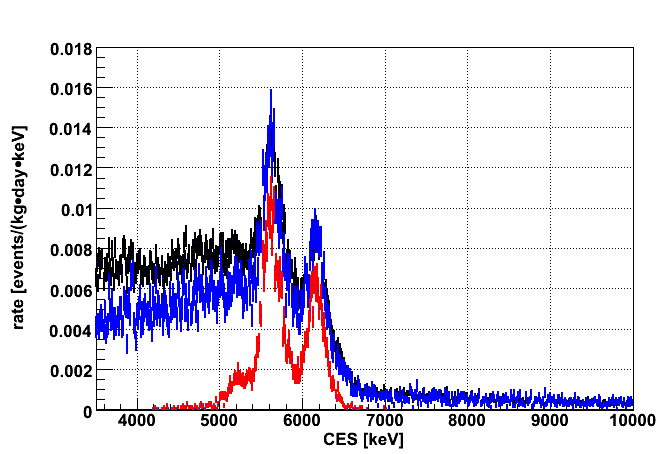
\includegraphics[width=0.475\linewidth]{plots/RnDC/CES_13sets_dru.png}
%\label{figCESalpha_1}}
%\subfigure[]{
%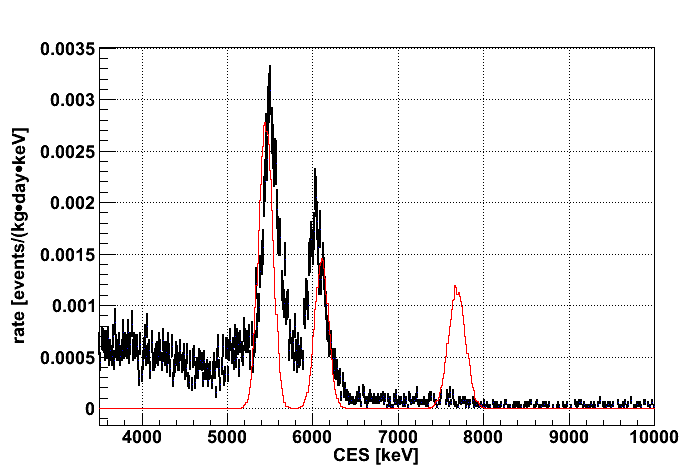
\includegraphics[width=0.475\linewidth]{plots/RnDC/MCdata_Rn222_2ndPeak.png}
%\label{figCESalpha_2}}
%\caption{Alpha peaks in combined energy scale (resolution 1.7\%), black - target volume, blue - FV 30kg, red - main alpha peaks. Data and MC, Rn-222 decay down to Po-210.}
%\label{figCESalpha}
%\end{figure}

